\documentclass[../main.tex]{subfiles}
\graphicspath{{\subfix{../images/}}}

\begin{document}

\subsection{Overview}
% High-level components and their interaction
A three-tier architecture consisting of a presentation tier, an application logic tier and a data tier is chosen for the e-Mall system, mainly due to the following reasons:
\begin{itemize}
    \item Module independence: the three tiers can be developed independently at the same time.
    \item Security: it guarantees major security, since clients cannot have direct access to the database.
    \item Re-use of data: the database can be re-used by other applications easily.
\end{itemize}

\begin{figure}[H]
    \centering
    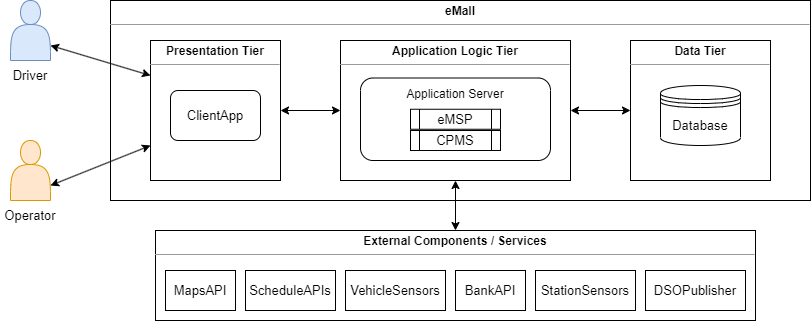
\includegraphics[width=0.95\textwidth]{images/Overview.png}
    \caption{High-level overview of the eMall system architecture}
    \label{fig:overview}
\end{figure}
\\
A description of the three tiers is reported below.
\begin{itemize}
    \item \textbf{Presentation tier}: it is the top-level tier of the designed mobile application with a graphical user interface. It interacts with the users by displaying information and collecting inputs from them, and it communicates with the application logic tier. 
    \item \textbf{Application logic tier}: this middle tier consists in the application server, which supports the system's functionalities by processing the data collected by the presentation layer and handling the operations concerning the database. In our case, it supports the activities of both eMSP and CPMS subsystems, and it also deals with various external components and services. 
    \item \textbf{Data tier}: it is responsible for persistent data storage, and it can be only accessed by the application server.
\end{itemize}


\subsection{Component view}
Here the component diagram offers a general view of the system's components and their interactions. In addition, all the components are presented and described. 
\begin{figure}[H]
    \centering
    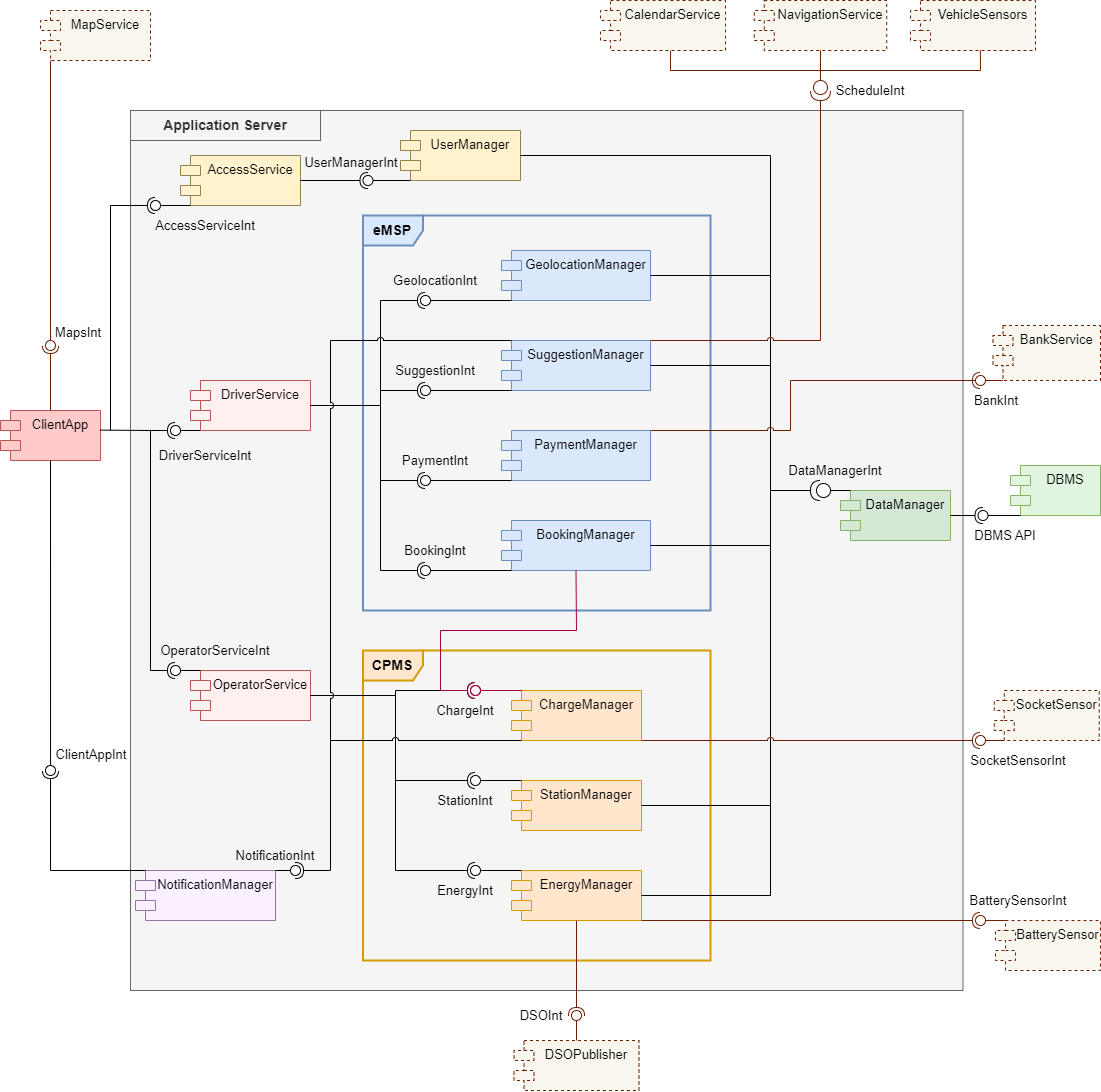
\includegraphics[width=0.98\textwidth]{images/ComponentDiagram.png}
    \caption{Component Diagram of the eMall system}
    \label{fig:component}
\end{figure}


\subsubsection{System Components}
The system's architectural components are:
\begin{itemize}
    \item \textbf{ClientApp} represents the mobile application client, and it generates views for the user based on the responses from the server. It communicates with the external MapService for map functionalities. 
    
    \item \textbf{AccessService} handles the registration process, the login process, and the modification of the account's personal data. It also gives the correct authorization role to the user after the successful completion of the authentication.\\
    \begin{figure}[h]
        \centering
        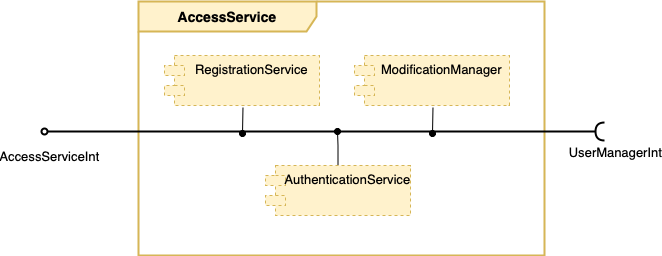
\includegraphics[width=70mm]{subcomponentDiagram/accessservice.drawio.png}
        \caption{Sub-components of AccessService component}
        \label{fig:subcomponent}
    \end{figure}\\
    It consists of the following sub-components:
    \begin{itemize}
        \item \textbf{RegistrationService} is responsible for the registration process of the user (only for Driver).
        \item \textbf{AuthenticationService} is responsible for the authentication process for both Driver and Operator. If the operation is successful, the user's login token is stored client-side in a encrypted way.
        \item \textbf{ModificationManager} manages the modification of data regarding the user's account.
    \end{itemize}
    \item \textbf{UserManager} interacts with DataManager, retrieving and storing user-related data for the creation of an account, the verification of credentials and the modification of account's personal information.

    \item \textbf{DriverService} handles the available operations for a driver: visualize the nearby charging stations and their external status, book a charge, start and end a charging process, pay for the received service, and receive charging suggestions. The user authorization is checked each time before accessing to the methods. 
    \item \textbf{GeolocationManager} is responsible for the visualization of the charging stations, along with their respective charging costs, special offers, and charging availabilities. It gets the necessary information about charging stations from DataManager.
    \item \textbf{BookingManager} deals with the procedures related to the operation of booking a charge. It allows the driver to book a charge, to start the charge according to the reservation, and to end the charge. The information about the driver account's linked vehicles is obtained from UserManager, and it interacts with DataManager to retrieve the charging station's availability, to register a new reservation and to update the reservation's status. Moreover, it communicates with ChargeManager to start and end the charging process at the chosen charging station.
    \item \textbf{PaymentManager} activates the payment process of the driver after the completion of a charge. It communicates with an external BankService to process the payment. 
    \item \textbf{SuggestionManager} is responsible of preparing the charging suggestions for the driver according to his schedule. The suggestions are made with respect to the stations' availability got from DataManager, and the user schedule, thanks to the information pulled periodically from the external APIs.
    
    \item \textbf{OperatorService} handles the available operations for a charging station's operator: check the status of the charging station, promote a special offer, modify the charging cost, modify the source of energy used for the charges, and acquire energy from DSOs. The user authorization is checked each time before accessing to the methods. 
    \item \textbf{StationManager} is responsible of visualizing the external and internal status of the charging station, and it allows the operator to modify the charging costs and to promote special offers. It interacts with DataManager to update the available costs and the offers. 
    \item \textbf{ChargeManager} allows to start and end a charging process at the station according to the reservation. It gets information about the vehicle connected to the charging column through SocketSensor.
    \item \textbf{EnergyManager} is responsible of modifying the energy source for charges, checking the level of batteries of the charging station, and handling the energy acquisition process. It communicates with the external DSOPublisher to get information about energy costs and to acquire energy from DSOs. Moreover, it updates the energy source status by interacting with DataManager. If batteries are present, it also deals with the BatterySensor of the station.

    \item \textbf{NotificationManager} sends the notifications generated by the server to the user's device. In particular, SuggestionManager uses it to send charging suggestions, and ChargeManager uses it to notify the user when the vehicle's battery is fully charged.
    
    \item \textbf{DataManager} handles the data requests of the other system components. According to the operation, it retrieves or stores proper information by interacting with the DBMS, making queries or updating it. 
    \item \textbf{DBMS} contains the system's persistent database with different schemas.

\end{itemize}


\newpage
\subsubsection{External Components}
On the other hand, the external components and services are:
\begin{itemize}
    \item \textbf{MapService} offers the possibility to visualize maps with the charging stations' location, and it also allows to search for specific addresses or station names. Its functionality of device localization requires a working GPS sensor of the mobile phone.
    \item \textbf{CalendarService} allows the system to get access to the driver's calendar information. 
    \item \textbf{NavigationService} allows the system to get access to the driver's navigation system, in order to know about his paths.
    \item \textbf{VehicleSensors} offers the access to the electric vehicle's sensors, and the system can acquire the battery level information of the vehicle in this way. 
    \item \textbf{BankService} handles the operation's payment with respect to the chosen method and the credit information inserted by the driver. The supported payment options are credit/debit cards and mobile payment systems such as PayPal, Apple Pay and Google Pay. 
    \item \textbf{SocketSensor} monitors the status of the electric vehicle connected to the charging column's socket. In particular, it is able to check the vehicle's number plate and its battery level in time.
    \item \textbf{BatterySensor} monitors the status of the batteries of the charging station, if present. 
    \item \textbf{DSOPublisher} handles the interactions with DSOs: it allows the system to know the energy costs published by the DSOs, and to acquire energy from them with respect to the chosen option.
\end{itemize}

\newpage
\subsubsection{Entity Relationship Diagram}
The high-level entity relationship diagram of the database is shown below. 
\vspace{3em}
    {\begin{figure}[H]
    \centering
    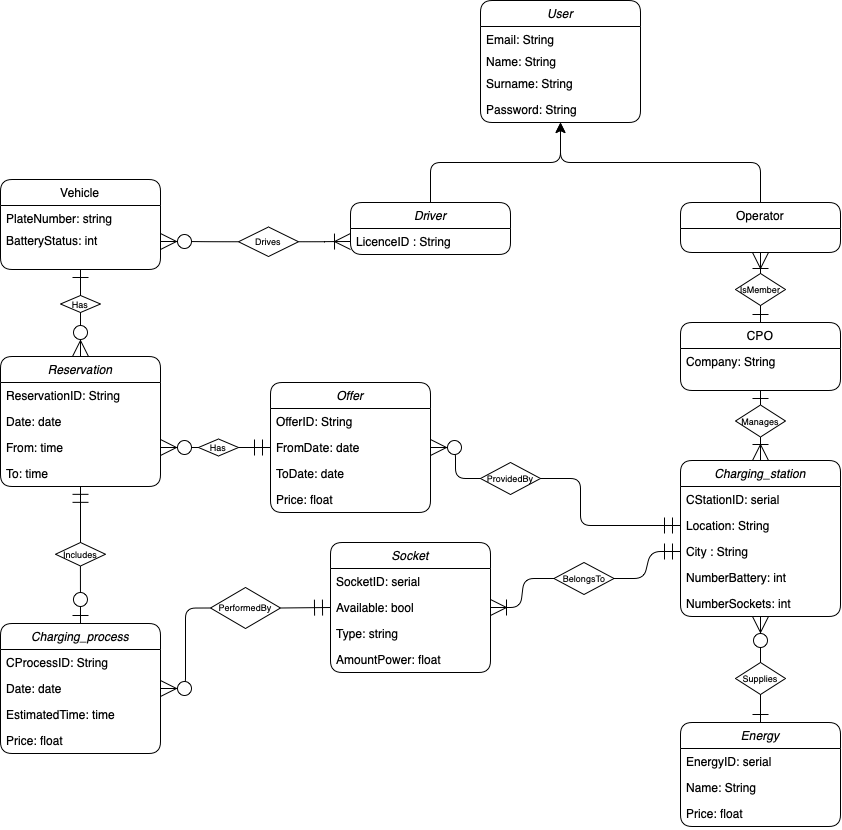
\includegraphics[width=0.95\textwidth]{images/ERDiagram.png}
    \caption{Entity Relationship Diagram of the e-Mall database}
    \label{fig:er}
    \end{figure}}
    
\newpage
\noindent
From the previous ER schema, it is possible to derive the following logical model: 
\begin{itemize}
    \item [] \textbf{Driver} (\underline{LicenceID}, \underline{Email}, Name, Surname, Password)
    \item [] \textbf{Operator} (\underline{Email}, Name, Surname, Password)
    \item [] \textbf{CPO} (\underline{Company})
    \item [] \textbf{ChargingStation} (\underline{CStationID}, Location, City, NumberSockets)
    \item [] \textbf{Energy} (\underline{EnergyID}, Name, Price)
    \item [] \textbf{Socket} (\underline{SocketID}, Available, Type, AmountPower)
    \item [] \textbf{Offer} (\underline{OfferID}, FromDate, ToDate, Price)
    
    \item [] \textbf{Vehicle} (\underline{PlateNumber}, BatteryStatus)
    \item [] \textbf{Reservation} (\underline{ReservationID}, Date, From, To)
    \item [] \textbf{ChargingProcess} (\underline{CProcessID}, Date, EstimatedTime, Price)
\end{itemize}





\newpage
\subsection{Deployment view}
In this section a deployment diagram of the system is presented, it describes the environments and tools used to build the eMall system. The communication protocols between the various parts are also specified.

\begin{figure}[H]
    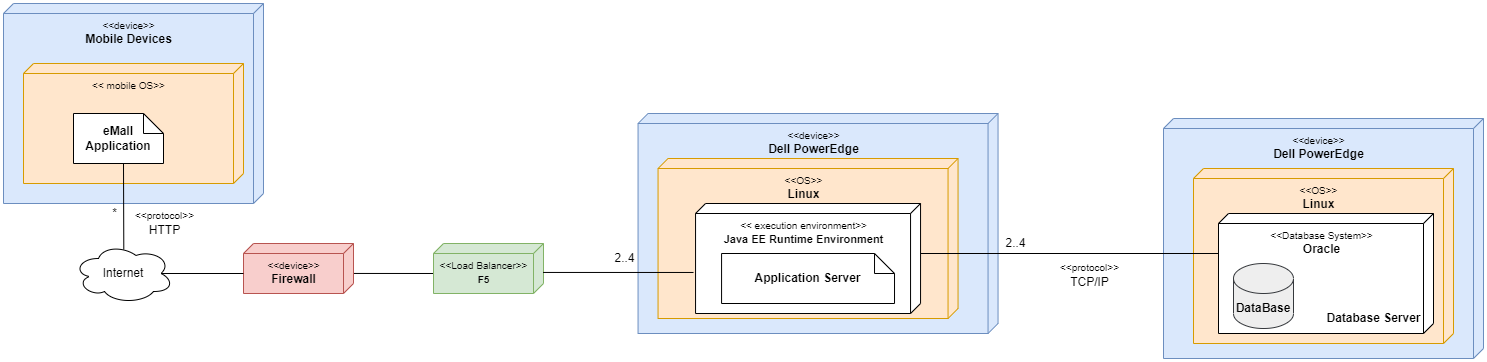
\includegraphics[width=1.05\textwidth]{images/DeploymentDiagram.png}
    \caption{Deployment Diagram}
    \label{fig:deploymentDiagram}
\end{figure}

\begin{itemize}
    \item \textbf{Mobile Devices} are smartphones and tablets where the Users (drivers and operators) install and run eMall Application. These devices need to connect to the system via Internet. The Client End will be separately developed for the different kind of operating systems, such as IOS, Android and HarmonyOS.
    \item \textbf{Firewall} manages the dataflow from clients to servers by filtering the packets from the Internet for security issues.
    \item \textbf{Load Balancer} distributes the workload among available resources to achieve availability and reliability. The idea is a load balancer with Least Connections method to balance the workload between the available application servers.
    \item \textbf{Application Server} contains all the application logic of the system and interacts with the Database Server. It should be replicated to increase reliability and availability. The Server device use Linux OS and the application server runs in a Java EE Runtime Environment, because it allows to develop distributed applications through standardized and modular components, with the aid of various integrated services. For example, the Persistence API can be used for connecting and manage the DBMS thanks to the object/relational mapping, and a REST API can be easily implemented for web services through JAX-RS.
    \item \textbf{Database Server} hosts the system’s Database, which is accessible through MySQL.
\end{itemize}

\subsection{Runtime view}
% You can use sequence diagrams to describe the way components interact to accomplish specific tasks typically related to your use cases
This section contains the runtime sequence diagrams about the eMall system's main functionalities, considering the use cases analyzed in the RASD. The diagrams describe the dynamics of the interactions among system's components.

\begin{itemize}
    \item Register a new account
    {
    \vspace{2em}
    \begin{figure}[H]
    \centering
    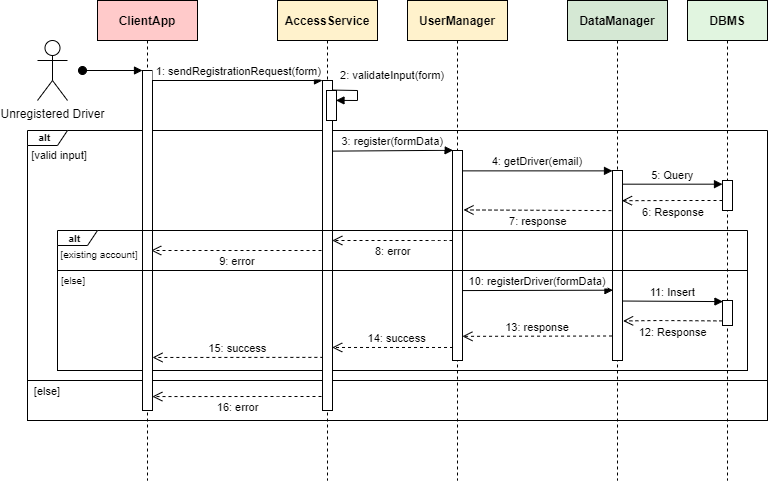
\includegraphics[width=\textwidth]{runtimeview/rv_registration.png}
    \caption{Runtime View of Driver Registration}
    \label{fig:rv_registration}
    \end{figure}}
    The sequence diagram above shows the driver registration process. The unregistered driver is on the Login page of the eMall application and he chooses to register an account. The registration form is displayed by clicking on the "Register" button. After filling the form, the driver clicks on "Confirm" and the registration request is sent to AccessService, which begins to handle the operation. An error message will be shown if the procedure fails, e.g. the input is invalid, or the email address is already associated to an account. Otherwise, the driver will see a success message.

    \newpage
    \item Login
    {
    \vspace{2em}
    \begin{figure}[H]
    \centering
    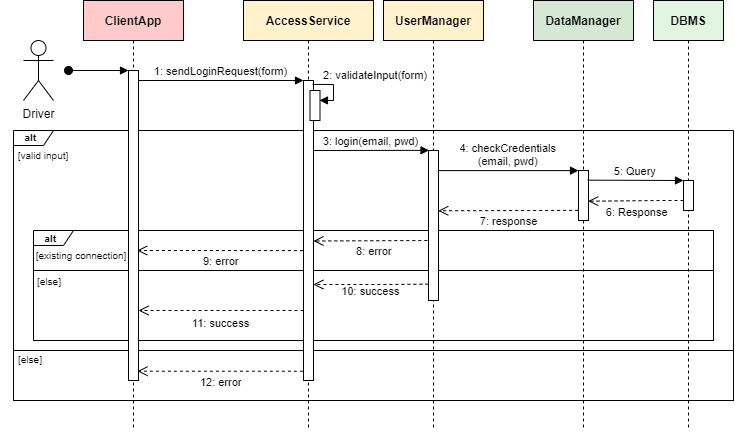
\includegraphics[width=\textwidth]{runtimeview/rv_login.png}
    \caption{Runtime View of User Login}
    \label{fig:rv_login}
    \end{figure}}
    The sequence diagram above shows the login process. The user (driver or operator) is on the Login page of the eMall application, and he clicks on the "Login" button. The request is sent to AccessService after filling and submitting the login form. If a success response is received, now the user is correctly authenticated and he is redirected to the corresponding Main Page according to his role.

    \newpage
    \item Add a vehicle to the Driver profile
    {
    \vspace{2em}
    \begin{figure}[H]
    \centering
    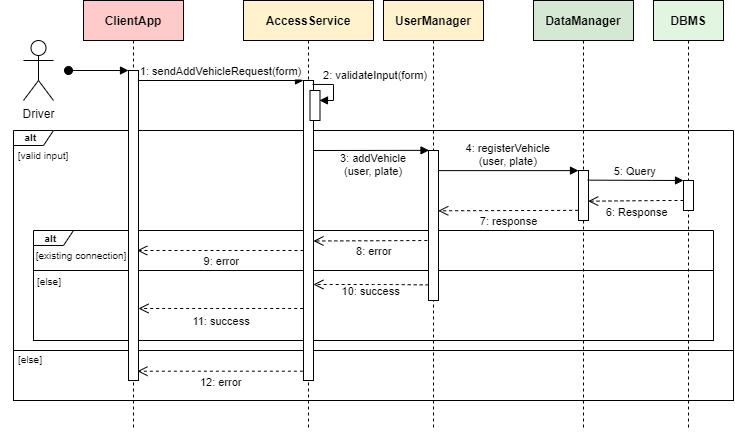
\includegraphics[width=\textwidth]{runtimeview/rv_addVehicle.png}
    \caption{Runtime View of adding a vehicle to the profile}
    \label{fig:rv_addVehicle}
    \end{figure}}
    The sequence diagram above shows an example of updating the account's personal information, more specifically we deals about adding a vehicle to the driver's profile. The driver is correctly logged in, and he finds the option to add a vehicle in his personal profile page. The request is processed by AccessService, which calls UserManager to complete the procedure. Then the vehicle is linked to the driver's account if the input data is valid and the vehicle has not been connected to this account yet. 

    \newpage
    \item Visualize charging stations nearby
    {
    \vspace{2em}
    \begin{figure}[H]
    \centering
    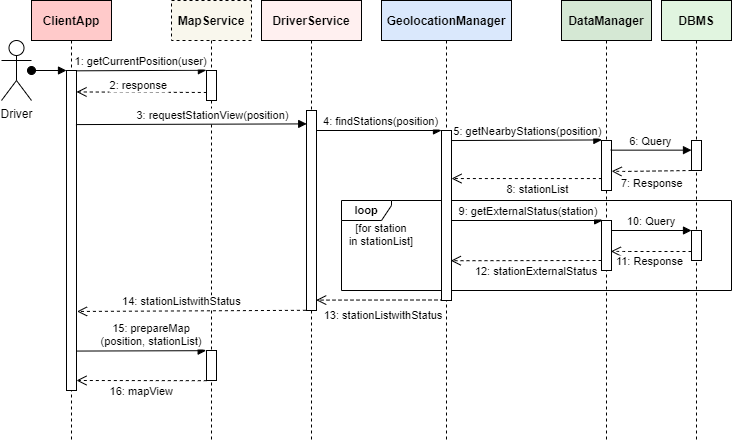
\includegraphics[width=\textwidth]{runtimeview/rv_visualizeStations.png}
    \caption{Runtime View of visualizing charging stations nearby}
    \label{fig:rv_visualize}
    \end{figure}}
    The sequence diagram above describes the process of visualizing nearby charging stations on the map. The application gets the device's current position through the external MapService, and DataManager makes query to the DBMS in order to find the nearby stations and their status. The retrieved information is processed by GeolocationManager and sent to the client, which asks MapService to prepare the view of the map.

    \newpage
    \item Book a charge
    {
    \vspace{2em}
    \begin{figure}[H]
    \centering
    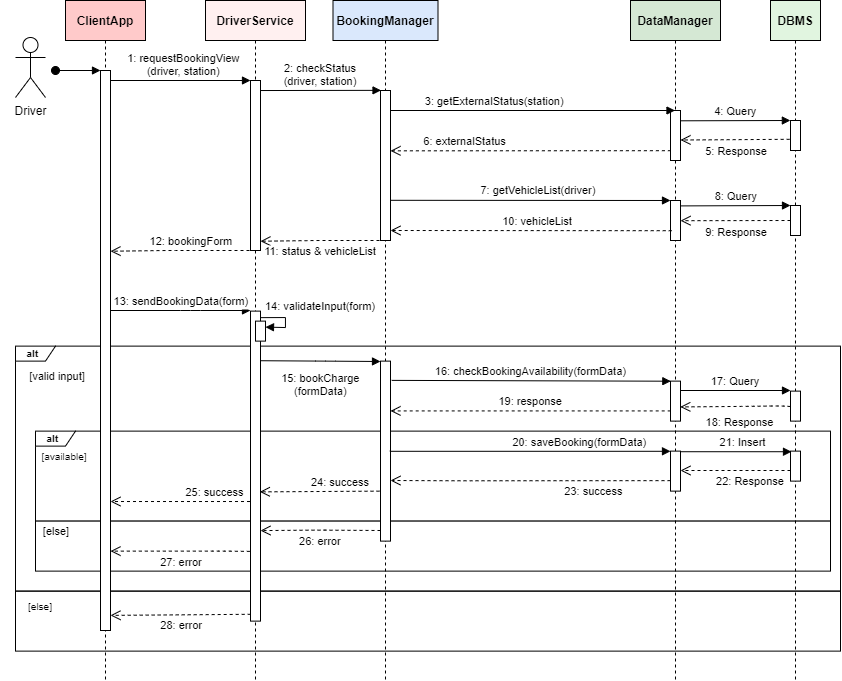
\includegraphics[width=\textwidth]{runtimeview/rv_bookCharge.png}
    \caption{Runtime View of booking a charge}
    \label{fig:rv_book}
    \end{figure}}
    The sequence diagram above describes the process of booking a charge. The logged driver chooses a charging station to initiate the booking process. BookingManager checks the external status of the selected station and the list of vehicles of the driver, and then a booking form is displayed. After submitting the form, BookingManager handles the registration of the reservation if the data is valid and the option is available.

    \newpage
    \item Start a charge
    {
    \vspace{2em}
    \begin{figure}[H]
    \centering
    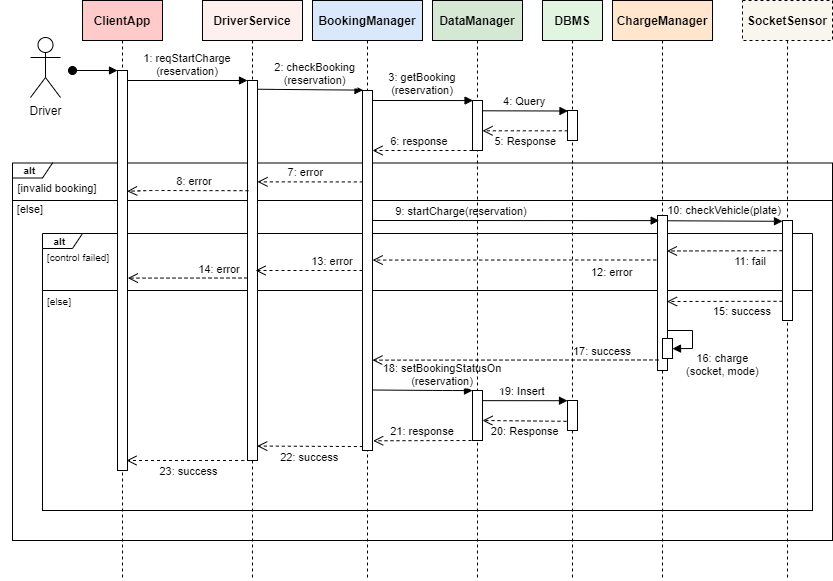
\includegraphics[width=\textwidth]{runtimeview/rv_startCharge.png}
    \caption{Runtime View of starting a charge}
    \label{fig:rv_start}
    \end{figure}}
    The sequence diagram above shows the procedure to start a charging process. The driver arrives at the charging station, plugs the vehicle in the assigned charging socket, and sends a start charge request from the eMall application on his device. BookingManager checks the validity of the reservation and asks ChargeManager to handle the charging process at socket level. If the vehicle has begun charging correctly, it becomes locked and the booking status is updated to "ON" in the database.

    \newpage
    \item Finish a charge
    {
    \vspace{2em}
    \begin{figure}[H]
    \centering
    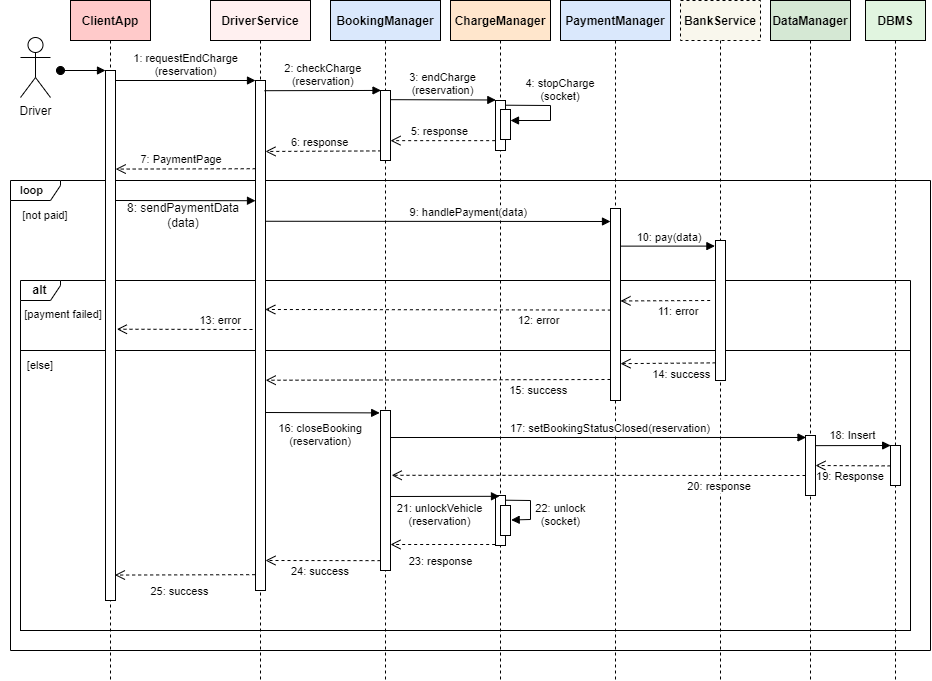
\includegraphics[width=\textwidth]{runtimeview/rv_endCharge.png}
    \caption{Runtime View of finishing a charge}
    \label{fig:rv_end}
    \end{figure}}
    The sequence diagram above shows the procedure to end a charging process. The driver receives the notification that the vehicle's battery is fully charged, and he arrives at the charging station. He confirms to end the charging process in the application. BookingManager checks the charging status and ChargeManager stops the power supply of the socket.
    \\
    Then the driver is asked to pay for the obtained service, and the payment is processed with the help of the external BankService. If the payment is successful, the booking status is updated to "CLOSED" and the vehicle is unlocked at this point.

    \newpage
    \item Suggest the driver to charge the vehicle
    {
    \vspace{2em}
    \begin{figure}[H]
    \centering
    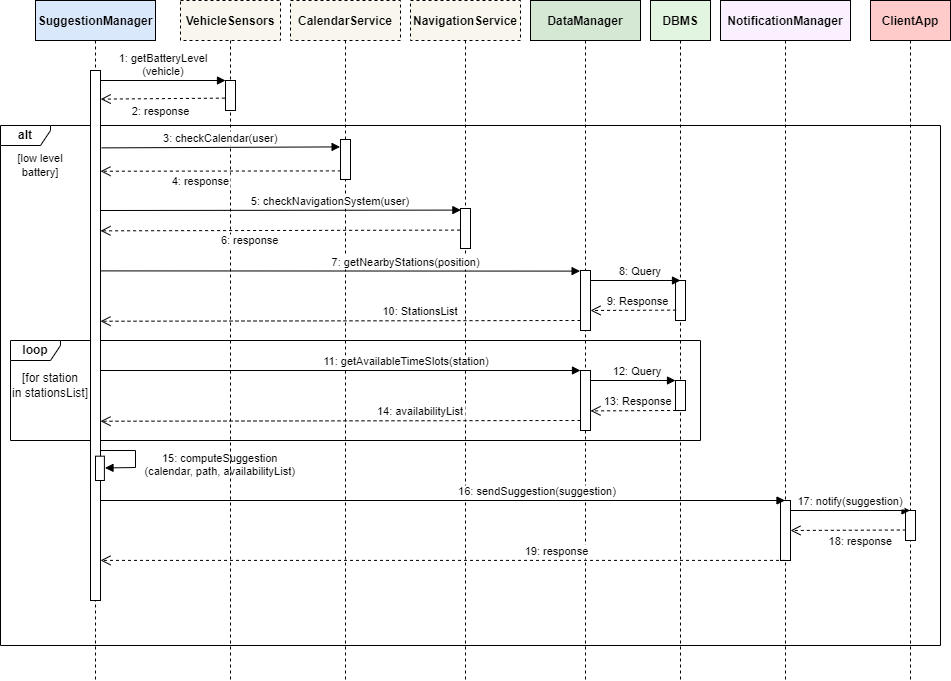
\includegraphics[width=\textwidth]{runtimeview/rv_suggest.png}
    \caption{Runtime View of charging suggestions}
    \label{fig:rv_suggest}
    \end{figure}}
    The sequence diagram above illustrates the process of making suggestions to the driver for the vehicle's charging. 
    \\
    SuggestionManager periodically checks the vehicle's battery status through VehicleSensors during the day. It retrieves information about the driver's schedule from CalendarService and NavigationService if the low level battery status is detected. In addition, it interacts with DataManager to find the nearest charging stations with the respective available time slots. Then it computes the best plans and sends the suggestions to NotificationManager, which notifies the Client Application.

    \newpage
    \item Check the overall status of charging station
    {
    \vspace{2em}
    \begin{figure}[H]
    \centering
    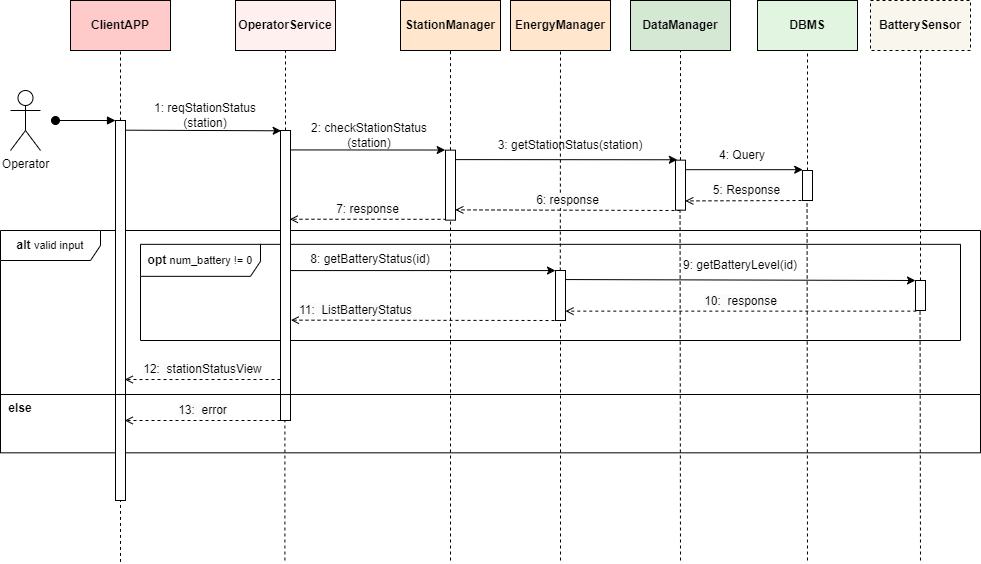
\includegraphics[width=\textwidth]{runtimeview/op_station.png}
    \caption{Runtime View of checking the charging station status}
    \label{fig:op_station}
    \end{figure}}
    The sequence diagram above shows the process that a logged operator checks the status of a chosen charging station. StationManager retrieves the information about the station stored in the database, while EnergyManager communicates with BatterySensor to get the level of the batteries in the station if they are present. Then the overall view is displayed to the operator. 

    \newpage
    \item Define a special offer
    {
    \vspace{2em}
    \begin{figure}[H]
    \centering
    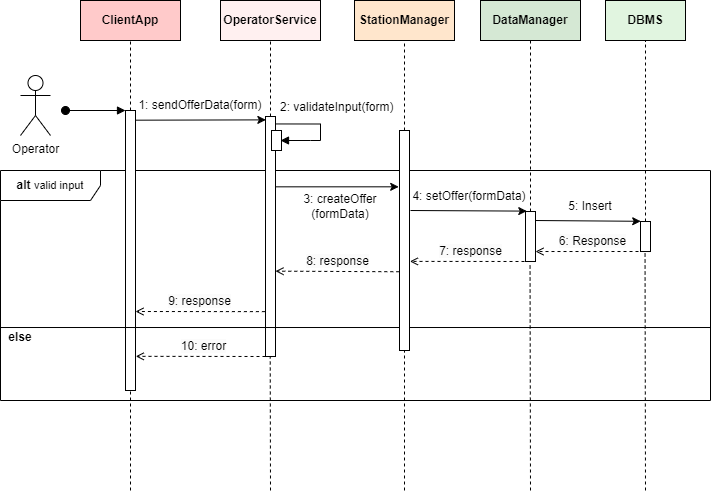
\includegraphics[width=\textwidth]{runtimeview/op_offer.png}
    \caption{Runtime View of defining a special offer}
    \label{fig:op_offer}
    \end{figure}}
    The sequence diagram above shows the process of defining a special offer for a chosen charging station. The operator submits the form with the required information (socket type, cost, start and end dates), and StationManager process it. If the input is valid, the offer is updated in the database.

    \newpage
    \item Modify the charge cost
    {
    \vspace{2em}
    \begin{figure}[H]
    \centering
    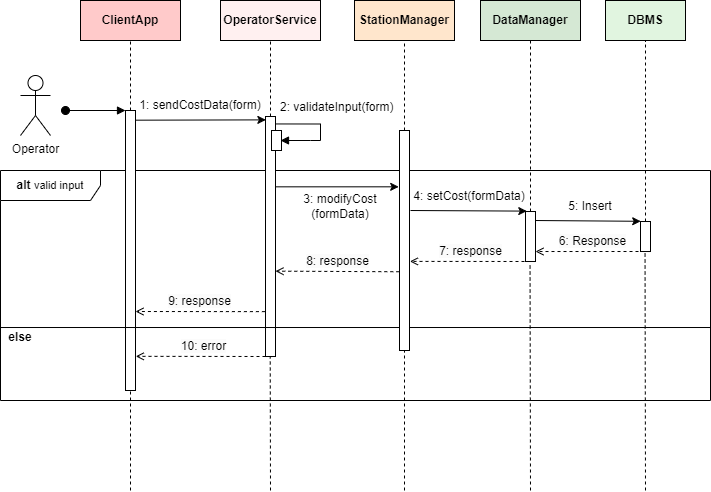
\includegraphics[width=\textwidth]{runtimeview/op_cost.png}
    \caption{Runtime View of modifying the charge cost}
    \label{fig:op_cost}
    \end{figure}}
    The sequence diagram above shows the process of modifying the charge cost of a chosen charging station. The operator submits the form with the required information (socket type and cost), which is processed by StationManager.
    

    \newpage
    \item Acquire energy from DSO
    {
    \vspace{2em}
    \begin{figure}[H]
    \centering
    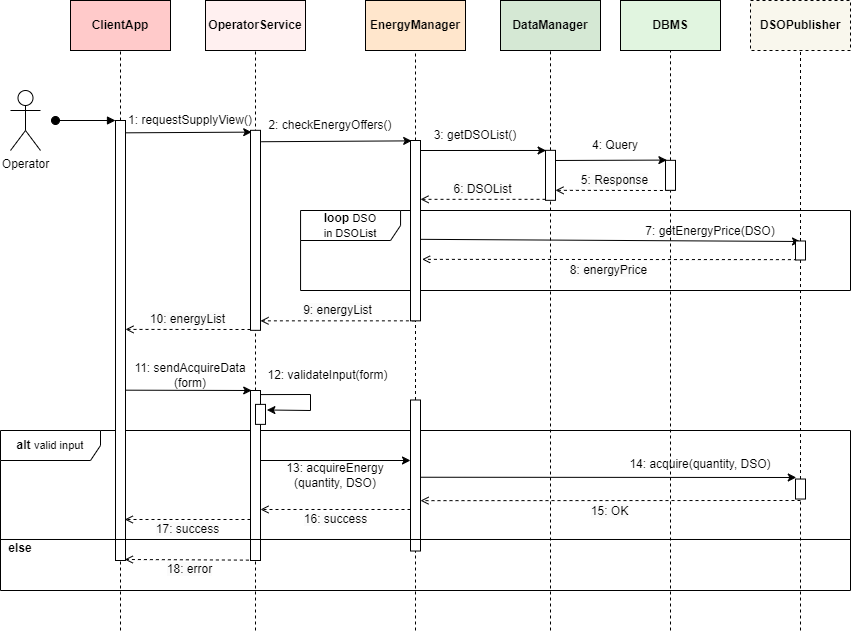
\includegraphics[width=\textwidth]{runtimeview/op_acquire.png}
    \caption{Runtime View of the energy acquisition process}
    \label{fig:op_acquire}
    \end{figure}}
    The sequence diagram above describes the process of acquiring energy from DSOs. EnergyManager communicates with DataManager to retrieve the list of DSOs, and it interacts with the external DSOPublisher to get the current energy offers of each DSO. If the operator wants to buy energy for the charging station, he submits the form for the energy acquisition which will be handled by EnergyManager and DSOPublisher.

    \newpage
    \item Modify the energy source for the charges
    {
    \begin{figure}[H]
    \centering
    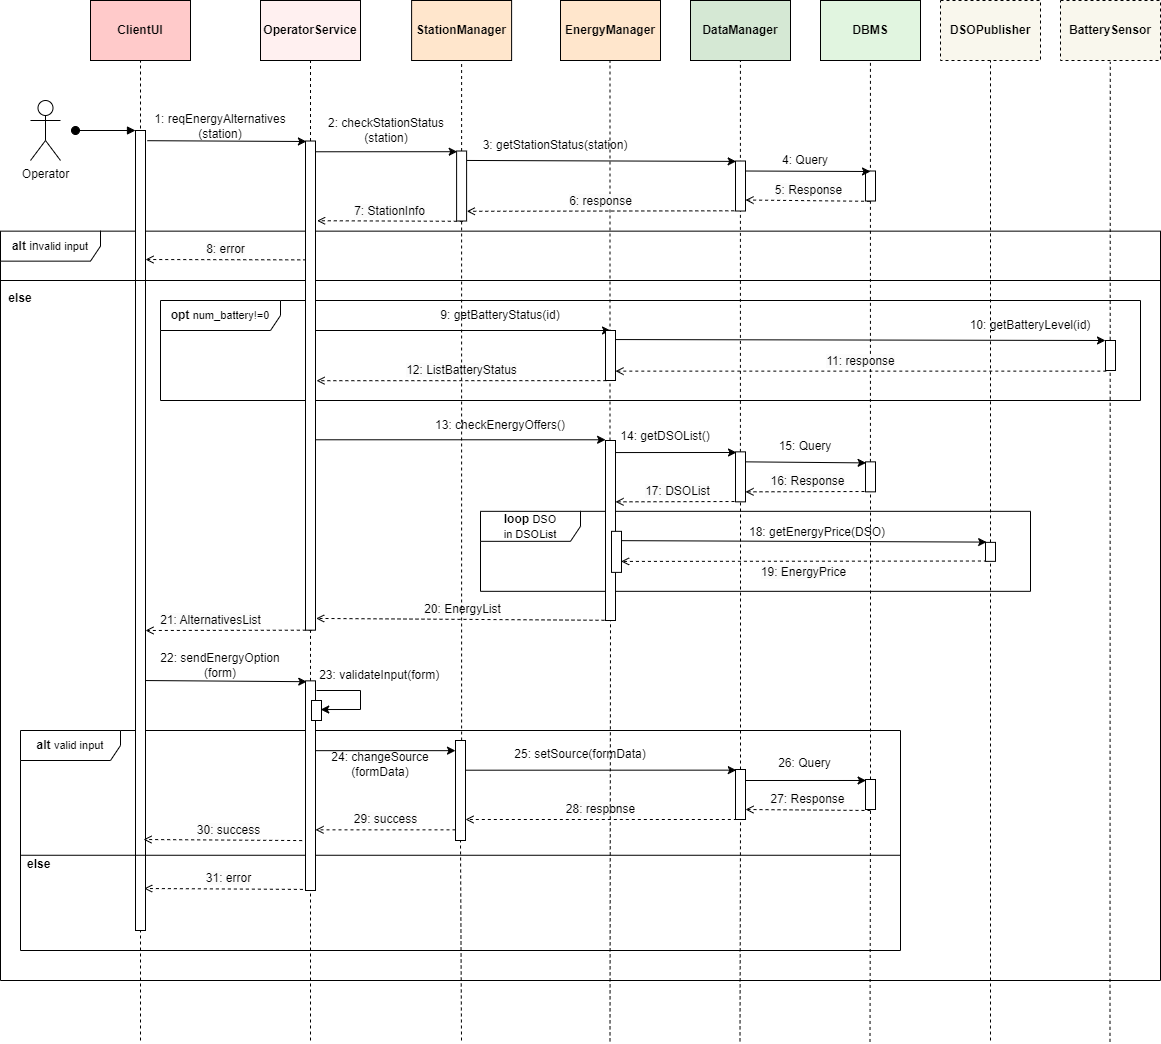
\includegraphics[width=\textwidth]{runtimeview/op_source.png}
    \caption{Runtime View of modifying the energy source for the charges}
    \label{fig:op_source}
    \end{figure}}
    The sequence diagram above shows the operation of modifying the energy source for charging the vehicles at the station. The logged operator requests the alternatives for energy supply, and the station status is checked. Then EnergyManager controls the level of batteries of the station and gets the current energy offers from DSOPublisher. The list of alternatives is then displayed to the operator. After choosing an option, the process of changing the energy source is handled by StationManager.
    
    
\end{itemize}


\newpage
\subsection{Component interfaces}
The component interfaces are presented in detail in the following part.
\begin{itemize}
    \item \textbf{AccessServiceInterface} is accessible from ClientApp.
    \begin{itemize}
        \item \textbf{sendRegistrationRequest(form)}: it takes as input the data filled in the account registration form, which includes the driver's name and surname, the email address, the driving licence number and the password. It returns a success message if the registration is correctly completed, otherwise an error message is shown.
        \item \textbf{validateInput(form)}: the data format of the form fields is checked. It returns False if the data is formatted wrongly, otherwise True.
        \item \textbf{sendLoginRequest(form)}: it takes as input the user login form containing the email address and the password. It returns a success or an error message.
        \item \textbf{sendLogOutRequest(email)}: it takes as input the user's email address and the password. It returns a success or an error message.
        \item \textbf{sendAddVehicleRequest(form)}: the number plate of the vehicle that the driver wants to add to the own profile is recorded and wrapped in a form along with the account identifier as the function's input. If the operation is successful, it returns a success message, otherwise the driver is informed of the error.
        \item \textbf{sendDelVehicleRequest(form)}: the number plate of the vehicle that the driver wants to delete from his own profile is recorded and wrapped in a form along with the account identifier as the function's input. If the operation is successful, it returns a success message, otherwise the driver is informed of the error. 
    \end{itemize}

    \item \textbf{UserManagerInterface} is accessible from AccessService, and it offers functionalities for the retrieval and the storing of user-related data in the database.
    \begin{itemize}
        \item \textbf{register(formData)}: it takes as input the registration request processed by AccessService, and it returns an error or a success message with respect to the registration's outcome.
        \item \textbf{login(email, pwd)}: it takes as input the email address and the password inserted by the user from AccessService, and it returns the authorization token for the user's current session if the login is correctly done, otherwise it returns an error.
        \item \textbf{logout(email)}: it takes as input the email address of the user and it returns an error or a success message with respect to the operation's outcome.
        \item \textbf{addVehicle(user, plate)}: it takes as input the driver identification and the number plate of the vehicle to be added. It returns an error or a success message with respect to the operation's outcome.
        \item \textbf{delVehicle(user, plate)}:it takes as input the driver identification and the number plate of the vehicle to be deleted. It returns an error or a success message with respect to the operation's outcome.
    \end{itemize}

    \item \textbf{DriverServiceInterface} is accessible from ClientApp after obtaining the authorization to access to the system's functionalities, and it exposes the operations available for a driver.
    \begin{itemize}
        \item \textbf{requestStationView(position)}: it takes as input the current position of the driver, and it returns the list of the nearby charging stations with their external status.
        \item \textbf{requestBookingView(driver, station)}: it takes as input the identification of the driver and the chosen charging station, and it returns the list of available booking options wrapped in a form.
        \item \textbf{sendBookingData(form)}: it takes as input the information filled in the charge booking form, and it returns a success or error message.
        \item \textbf{requestStartCharge(reservation)}: it takes as input the identification of the reservation made by the driver, and it returns a success or error message.
        \item \textbf{requestEndCharge(reservation)}: it takes as input the identification of the reservation made by the driver, and it returns the payment page if the charge successfully stops.
        \item \textbf{sendPaymentData(data)}: it takes as input the payment related data inserted by the driver, and it returns a success or error message.
        \item \textbf{validateInput(form)}: it takes as input the form data and validates its format. It returns False if the data has wrong format, and True if it is correctly formatted.
    \end{itemize}

    \item \textbf{GeolocationInterface} is accessible from DriverService, and it handles the functionality of visualizing the nearby charging stations along with their external status. 
    \begin{itemize}
        \item \textbf{findStations(position)}: it takes as input the current position of the driver, and it returns a list of charging stations with their external status.
    \end{itemize}

    \item \textbf{BookingInterface} is accessible from DriverService, and it offers the functionalities related to the charge booking. 
    \begin{itemize}
        \item \textbf{checkStatus(driver, station)}: it is involved in the preparation of the booking form for the driver. The input consists of the driver and the chosen station, while the return object includes the external status of the chosen charging station and the list of vehicles associated to the driver's account.
        \item \textbf{bookCharge(formData)}: its input is the data contained in the booking form, and it returns a success or an error message.
        \item \textbf{checkBooking(reservation)}: its input is the ongoing reservation's identifier, and it returns a success or an error message.
        \item \textbf{checkCharge(reservation)}: its input is the ongoing reservation's identifier, and it returns the operation summary with the value of its cost. 
        \item \textbf{closeBooking(reservation)}: its input is the ongoing reservation's identifier, and it returns a success or an error message.
    \end{itemize}

    \item \textbf{SuggestionInterface} offers the possibility to create charging suggestions for drivers. It is accessible from DriverService.
    \begin{itemize}
        \item \textbf{computeSuggestion(calendar, path, availabilityList)}: it computes the best suggestions according to the parameters, which are the driver's calendar schedule, the navigation path, and the list of availabilities of the charging stations. It returns a list containing suggestions.
    \end{itemize}

    \item \textbf{PaymentInterface} is accessible from DriverService.
    \begin{itemize}
        \item \textbf{handlePayment(data)}: it takes as input the payment data inserted by the driver, and it returns a success or error message.
    \end{itemize}

    \item \textbf{OperatorServiceInterface} is accessible from ClientApp after obtaining the authorization to access to the system's functionalities, and it exposes the operations that an operator is allowed to perform. 
    \begin{itemize}
        \item \textbf{requestStationStatus(station)}: it takes as the input the station to consider, and it returns an object encapsulating the external and internal status of the selected station.
        \item \textbf{sendOfferData(form)}: it takes as input the data contained in the offer creation form. It returns a success message if the operation is completed, otherwise an error message is displayed.
        \item \textbf{validateInput(form)}: it checks the validity of the data contained in the input form. The return value is True if it does not find errors, otherwise it is False.
        \item \textbf{requestSupplyView()}: it returns the list of energy costs published by DSOs. 
        \item \textbf{sendAcquireData(form)}: it takes as input the data contained in the energy acquisition form, and it returns a success or an error message.
        \item \textbf{sendCostData(form)}: its input is the data contained in the form for the modification of the charge cost, and it returns a success or an error message.
        \item \textbf{requestEnergyAlternatives(station)}: it takes as input the station for which the operator wants to modify the energy source used for the charging operations, and it returns the list of available energy sources for that charging station. 
        \item \textbf{sendEnergyOption(form)}: its input is the chosen option to modify the energy source used for the charges, wrapped in a formData format along with the station's identifier. At the end of the operation, a success or an error message is returned.
    \end{itemize}

    \item \textbf{ChargeInterface} handles the charging process at the station according to the driver's reservation, and it offers the possibility to the eMSP to access to its functionalities from BookingManager.
    \begin{itemize}
        \item \textbf{startCharge(reservation)}: it takes as input the reservation made by the driver, and it returns a success or an error message.
        \item \textbf{charge(socket, mode)}: it takes as input the socket assigned for the charge and the charging mode, and it returns True if the operation correctly begins, otherwise False. 
        \item \textbf{stopCharge(socket)}: it takes as input the socket assigned for the charge. The return value is True if the power supply correctly stops, False otherwise.
        \item \textbf{unlockVehicle(reservation)}: it takes as input the reservation made by the driver, and it returns a success or an error message. 
        \item \textbf{unlock(socket)}: it takes as input the socket where the vehicle is plugged in. It returns True if the vehicle is successfully unlocked, False otherwise.
    \end{itemize}

    \item \textbf{StationInterface} is accessible from OperatorService. 
    \begin{itemize}
        \item \textbf{checkStationStatus(station)}: the input is the charging station the operator wants to check the status, and it outputs the status information of the station.
        \item \textbf{createOffer(formData)}: its input consists in the data necessary for the creation of a new offer. It returns a success message or an error message.
        \item \textbf{changeSource(formData)}: its input is the data necessary for the modification of the energy source used for the charges. At the end of the operation, it returns a success or an error message.
        \item \textbf{modifyCost(formData)}: 
    \end{itemize}

    \item \textbf{EnergyInterface} is accessible from OperatorService.
    \begin{itemize}
        \item \textbf{getBatteryStatus(id)}: its input is the battery's identification number, and it returns the value of the battery level.
        \item \textbf{checkEnergyOffers()}: it returns a list of energy costs published by DSOs.
        \item \textbf{acquireEnergy(quantity, DSO)}: it takes as input the quantity of energy and the DSO provider from which to acquire energy, and it returns a success message or an error message.
    \end{itemize}

    \item \textbf{DataManagerInterface} is accessible from the components which requires the retrieval and the storage of information in the database, and its methods are meant to send queries and insertions to the DBMS. 
    \begin{itemize}
        \item \textbf{getDriver(email)}: it finds the driver associated to the input email address.
        \item \textbf{registerDriver(formData)}: it registers a new account for the driver, with the information given by the formData. It returns a success or an error message.
        \item \textbf{checkCredentials(email, pwd)}: it checks the validity of the email address - password combination in the database. The return value is True if the combination is correct, otherwise False.
        \item \textbf{registerVehicle(user, plate)}: it associates the vehicle identified by the number plate to the driver's account.  It returns a success or an error message.
        \item \textbf{getNearbyStations(position)}: it returns the list of stations within a certain range of the given position. 
        \item \textbf{getExternalStatus(station)}: it returns the external status information of the chosen station.
        \item \textbf{getAvailableTimeSlots(station)}: it returns a list containing the available time slots of the chosen station.
        \item \textbf{checkBookingAvailability(formData)}: it checks the possibility of doing the reservation with respect to the input information.
        \item \textbf{saveBooking(formData)}: it stores the reservation in the database with respect to the input information.
        \item \textbf{getVehicleList(driver)}: it returns the list of vehicles associated to the given driver.
        \item \textbf{getBooking(reservation)}: it retrieves the reservation according to the given information.
        \item \textbf{setBookingStatusOn(reservation)}: it sets the input reservation's status to ON (vehicle charging), and it returns True if the operation is successful.
        \item \textbf{setBookingStatusClosed(reservation)}: it sets the input reservation's status to CLOSED (reservation ended and paid). It returns True if the operation is successful.
        \item \textbf{getStationStatus(station)}: it returns the overall status information of the chosen station.
        \item \textbf{setOffer(formData)}: it registers a new offer with respect to the input information. It returns a success or error message.
        \item \textbf{getDSOList()}: it returns the list of the available DSOs.
        \item \textbf{setSource(formData)}: it modifies the energy source option for the selected charging station. It returns a success or error message.
        \item \textbf{setCost(formData)}: it modifies the energy cost for the selected charging station. It returns a success or error message.
    \end{itemize}

    \item \textbf{NotificationInterface}: it is accessible from SuggestionManager and ChargeManager, and it aims to deliver notification to the user's mobile device.
    \begin{itemize}
        \item \textbf{sendSuggestion(suggestion)}: it sends the input suggestion to the destination user interface. 
        \item \textbf{sendNotification(notification)}: it sends the input notification to the destination user interface.
    \end{itemize}

    \item \textbf{ClientAppInterface}: it is accessible from NotificationManager with the objective to show the notification to the user.
    \begin{itemize}
        \item \textbf{notify(message)}: it takes as input the message that the system wants to send to the user's device.
    \end{itemize}
\end{itemize}

\noindent
From the other hand, the interfaces of the external components and sensors are:
\begin{itemize}
    \item \textbf{MapsInterface}: it provides localization and map functionalities to ClientApp.
    \begin{itemize}
        \item \textbf{getCurrentPosition(user)}: it returns the current position of the user's device. 
        \item \textbf{prepareMap(position, stationList)}: it returns the map view, on which the given position and the stations' location are highlighted.
    \end{itemize}

    \item \textbf{SocketSensorInterface}: it is accessed by ChargeManager and it offers the possibility to check the status of the vehicle connected to the socket.
    \begin{itemize}
        \item \textbf{checkVehicle(plate)}: it verifies the identity of the connected vehicle by checking its plate number.
        \item \textbf{checkVehicleBattery()}: it returns the battery level of the connected vehicle.
    \end{itemize}

    \item \textbf{BankInterface}: it is accessed by PaymentManager.
    \begin{itemize}
        \item \textbf{pay(data)}: it takes as input the payment data of the driver. After executing the operation, it returns an error message or a success message.
    \end{itemize}

    \item \textbf{BatterySensorInterface}: it is accessible from EnergyManager.
    \begin{itemize}
        \item \textbf{getBatteryLevel(id)}: it returns the power level of the battery indicated by the input identification number. 
    \end{itemize}

    \item \textbf{DSOPublisher}: it is accessible from EnergyManager.
    \begin{itemize}
        \item \textbf{getEnergyPrice(DSO)}: it returns the energy cost published by the chosen DSO. 
        \item \textbf{acquire(quantity, DSO)}: it takes as input the quantity of energy to acquire, and the DSO from which the operator wants to acquire energy. It returns a success message or an error message.
    \end{itemize}

    \item \textbf{ScheduleInterface}: it is accessible from SuggestionManager, and it offers the possibility to check the driver's schedule.
    \begin{itemize}
        \item (VehicleSensors) \textbf{getBatteryLevel(vehicle)}: it returns the battery level of the input vehicle.
        \item (CalendarService) \textbf{checkCalendar(user)}: it returns the list of today's user activities registered in the calendar. 
        \item (NavigationService) \textbf{checkNavigationSystem(user)}: it returns the user's path indicated in the navigation system.
    \end{itemize}
\end{itemize}



\subsection{Selected architectural styles and patterns}
% Explain which style/patterns are used, why, and how
\subsubsection{Three-tier architecture}
As described in Section 2.1, we adopt the three-tier architecture for the eMall system for keeping apart the application logic from the data layer. In particular, the presentation tier represents a thin client model because it does not contain heavy operations which requires complex logic, it only handles the tasks for the visualization of different views. 
\\
On the other hand, in order to realize the separation of concerns, the middle-tier Application Server contains all the application logic, and it handles the operations by interacting with the presentation tier and the data tier.


\subsection{Other design decisions}

\subsubsection{Relational Database}
In the e-Mall system, all the persistent data is stored in the database. For data management, we make use of a Relational DBMS. It guarantees the ACID properties of transactions, which are important for the system. In fact, multiple users can access the database to retrieve information at the same time and even if data is being updated. It ensures data integrity by verifying that the data necessary for creating the relationships are actually present, and it also assures data accuracy, avoiding duplicates so that data are defined and well organized. Lastly, data is secure as Relational Database Management System allows only authorized users to directly access the data. No unauthorized user can access the information.

\subsubsection{Stateless web service}
The choice of Java EE for the implementation of the backend allows to use JAX-RX for creating REST web services, which is stateless: the server's response do not rely on the previous requests sent by the client. A stateless application is more scalable, and it requires less server-side storage. 





\end{document}